% Identifying Early Heart Disease Risk Factors with Data Science
% Jacob Sánchez Pérez (jacob@san.contact)
% Data Science (CO3722)
% University of Central Lancashire

\documentclass[a4paper,12pt]{article}

% Links
\usepackage{hyperref}

% PDF Metadata
\hypersetup{
    hidelinks,
    pdftitle={Identifying Early Heart Disease Risk Factors with Data Science},
    pdfauthor={Jacob Sánchez}
}

% Code
\usepackage{minted}

% Referencing and more
\usepackage[british]{babel}
\usepackage{csquotes}
\usepackage[style=apa,backend=biber]{biblatex}

% Images
\usepackage{graphicx}
\graphicspath{ {./figures/} }

% Graphs
\usepackage{pgfplots}
\pgfplotsset{width=10cm,compat=1.9}
\usepgfplotslibrary{external}
\tikzexternalize

\title{Identifying Early Heart Disease Risk Factors with Data Science}
\author{Jacob Sánchez Pérez\\ University of Central Lancashire\\\texttt{jsanchez-perez@uclan.ac.uk}}
\date{}

\addbibresource{references.bib}

\begin{document}

\maketitle


\section{Introduction}

% PROMPT
% This section will introduce your project, your business, specific Use Case and potential source of a dataset for analysis.

% NOTES
% The business I have chosen is healthcare

Data science applies different methods in order to solve relevant problems and
make predictions \parencite[78]{Waller2013}.
One industry that can benefit from data science is the healthcare industry.
By improving productivity, public spending can be significantly reduced \parencite{oecd2010health}.
McKinsey estimated that data analytics can reduce healthcare expenses by up to
\$450 billion annually in the U.S.\parencite{Groves2013}.
Data science can be used to process the massive amounts of electronic health
records that exist, including physician notes, medical records, patient scans,
and patient sensor data \parencite{Adam2017, Dalianis2015}.
However, this data is not readily available due to patient privacy.
Areas in healthcare that could have the most impact include early detection of
diseases, precision medicine, optimisation of workflows, value-based healthcare,
infection prevention and control, and clinical research \parencite[9]{Consoli2019}.

This report is centred around the application of data science to identify early
risk factors of diseases.
Prompt identification of risk factors of fatal diseases can be quite beneficial
to the healthcare industry.
For instance, Coronary Heart Disease (CHD) was found to have a total annual
burden of £7.06 billion in the UK, the highest for any disease \parencite{Liu2002}.
This report will review in detail the process of data analysis, from locating a
data source, processing the data, and finally visualising and interpreting the results.

\section{Data Science for Healthcare}

% PROMPT
% This section will relate specifically to your business and Use Case and their approach or potential application for the use of data science.
% This will cover the challenge of acquiring or using specific data sources for your Use Case, approaches to data processing, description of proposed machine learning  algorithms and their design, opportunities for data visualisation and the methods for analysing/interpreting the data required to gain business competitive advantage.

\subsection{Challenges}

There exist several limitations to the data freely available for analysis.
As \textcite[2]{Dalianis2015} points out, this is mainly due to sensitive data
in medical records.
A survey found that the two biggest perceived obstacles towards obtaining
healthcare data were legal issues and data standardization \parencite{Kim2019}.

\subsubsection{Privacy Concerns}

The General Data Privacy Regulation (GDPR) in the E.U. and the Health Insurance
Portability and Accountability Act (HIPAA) in the U.S., protect data that can
identify a patient \parencite{Iyengar2018}.
GDPR requires explicit consent of the subject to process personal data.
Obtaining consent results impractical in big data analytics.
However, data can be processed for purposes such as research and analysis as
long as it is pseudonymised.
Pseudonymisation (de-identification) consists of replacing or removing direct
identifiers, such as names, phone numbers, and other identifying data \parencite{Hintze2018}.
Nowadays, de-identification can be performed through neural networks \parencite{Dernoncourt2016}.
However, no method is perfect and this is still a limiting factor in healthcare data availability.

\subsubsection{Processing Concerns}

In addition to the legal issues, data processing can be a major obstacle.
In particular, clinical notes can contain misspelled words, medical jargon,
and non-standard words \parencite{Dalianis2015}.
Furthermore, data is oftentimes collected from systems with incompatible formats
\parencite[34]{Consoli2019}.
Therefore significant preprocessing will be necessary before analysing the data.

\subsection{Data Sourcing}

\subsubsection{Healthcare Data Sources}

A selection of anonymised datasets that have been widely used in research due to
their high availability and relaxed access policy are listed below \parencite{Dalianis2015}.

\paragraph{MIMIC-II} A collection of data from ICU patients,
spanning 7 years and ~27,000 patient admissions.
The dataset contains patient demographics, intravenous medication drip rates,
laboratory test results, and physiological waveforms recorded at bedside.
The dataset can be accessed after registration free of charge \parencite{Lee2011}.

\paragraph{MIMIC-III} A successor to \textit{MIMIC-II}, it spans more than a
decade and \textgreater 50k patient admissions.
It contains demographics, notes and reports, tests, along with bedside monitoring data.
As its predecessor, access merely requires registration \parencite{Johnson2016}.

\paragraph{THIN} It is an ongoing dataset which begins in 1994, and represents
6\% of the UK population.
It contains records from general practices.
The dataset can only be accessed by those with special authorisation,
such as research organisations \parencite{Lewis2007}.

\paragraph{n2c2} Formerly known as \textit{i2b2} , it is a collection of datasets
of topics including smoking, obesity, medication, and heart disease,
The dataset requires registration and access request approval, yet is free of cost.

\subsubsection{Dataset Choice}

For the purpose of this report, the \textit{n2c2} dataset was chosen over the
other sources for its manageable size and ease of use.
Bigger datasets have the issue of becoming difficult to work with in consumer hardware,
since the records have to be pre-processed in a extensively to be able to use them.
Finally, the \textit{n2c2} datasets have the added benefit of being topic-focused,
which means that each dataset has been constructed with a particular health concern
or topic in mind.
From the different datasets contained in the \textit{n2c2} collection,
the one focusing in heart disease was selected, since heart disease is one of
the biggest public health concerns globally.
Additionally, there are several known risk factors for heart disease, which will
allow validation of the results \parencite{Kannel2002}.

The \textit{n2c2} heart disease dataset contains 1304 records which represent 296
diabetic patients \parencite{Kumar2015}.
After a request for access was filed and approved, the dataset was ready to be
analysed.


\subsection{Data Processing Techniques}

\subsubsection{De-identification}

De-identification techniques will not be covered here,
as the available datasets have been de-identified beforehand.
However, for the specific task of de-identification of the dataset in question,
\textcite{Yang2015} can be consulted (Figure \ref{fig:deid}).

% Kalman Filter Diagram
\begin{figure}[h]
\centering
\scriptsize
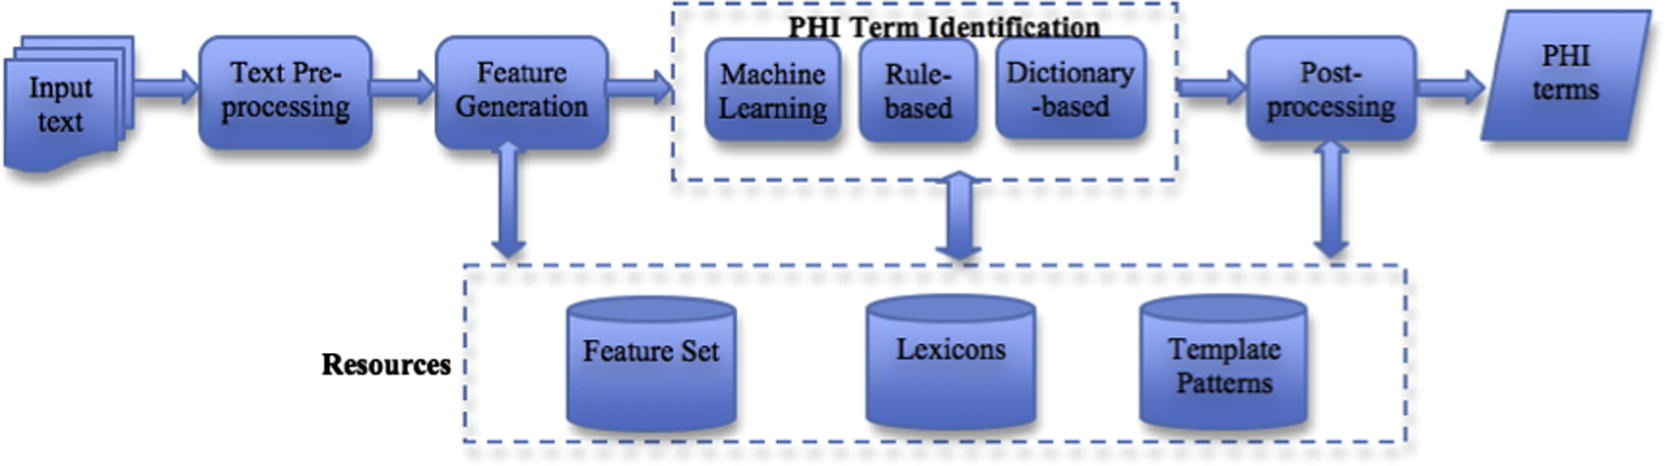
\includegraphics{deid}
\caption{De-identification Approach by \textcite{Yang2015}}
\label{fig:deid}
\end{figure}

\subsubsection{Data Cleaning}

Before attempting to perform any data analytics, it is a good idea to verify the integrity and quality of the dataset. Factors that can affect the quality of a dataset include: missing values, misspellings, duplicates, and mixed formats \parencite{Chu2016}. These can present themselves as outliers, values that are more than two standard deviations away from the mean \parencite{Hellerstein2008}. \textcite{Hellerstein2008} mentions robust estimators, resampling, and exploratory data analysis as ways to detect outliers in order to improve the data quality. While this may account for quantitative data, such as integers and floating point numbers, categorical variables must also be taken care of. Categorical data are words or names that \textquote[{\cite{Hellerstein2008}}]{assign data into categories or groups}, such as \textquote{dog} and \textquote{canine}.
While this is usually handled by deduplication, \textcite{Cerda2018} described an approach that encodes the similarity between categories, showing gains in performance.

\subsubsection{Text and Strings Specifics}

One of the most common ways to represent text for machine learning purposes is called \textit{bag-of-words}.
It consists of keeping a record of every unique word in the text, along with the number of times it is used.
Everything else, such as structure, formatting, and punctuation is discarded \parencite[327]{Mueller2017}.
There are additional measures that can improve the quality of data such as \textit{stopwords} (discarding frequent words) \parencite[327-336]{Mueller2017}, and \textit{term frequency–inverse document frequency} (rescale features by their expected importance);
as well as ways to improve the \textit{bag-of-words} technique, such as n-grams, stemming and lemmatization \parencite[339,344]{Mueller2017}.

Since patient records, such as the ones contained in the 
In healthcare, some techniques that might improve the quality of free-text data may include detection of negation and spelling mistakes, abbreviation normalisation, and named entity recognition \parencite{Dalianis2015}.

\subsection{Machine Learning}

Before investigating the different algorithms that can be used to analyse data, a quick distinction should be drawn between different types of machine learning algorithms.

\begin{itemize}
 \item Supervised Learning
 \item Unsupervised Learning
 \item Semisupervised Learning
 \item Reinforcement Learning
 \item Deep Learning
\end{itemize}

Supervised learning happens when the model is trained on labelled data, that is, data that has been classified beforehand.
Conversely, in unsupervised learning all data is unlabelled and the model deduces the structure from it. In semisupervised learning, data can be labelled or unlabelled.
Reinforcement learning happens when the model is conditioned externally \parencite[11]{Ibrahim2021}.
Finally, deep learning involves a series of layers that process the data and feed into one another \parencite[13]{Ibrahim2021}.

\subsection{Supervised Learning Algorithms}

\textcite{Jothi2015} outlined some of the classification algorithms commonly used in healthcare data analysis, briefly described next. All of them need exclusively labelled data and are thus considered supervised learning algorithms.

\begin{description}
    \item[Decision Tree] \textquote[{\cite[70]{Mueller2017}}]{They learn a hierarchy of if/else questions, leading to a decision}.
    \item[K-nearest Neighbour] Stores the training dataset, then to make a prediction it \textquote[{\cite[35]{Mueller2017}}]{finds the closest data points in the training dataset}.
    \item[Logistic Regression] Statistical model that \textquote{describes the relationship between a qualitative dependent variable and an independent variable}, making binary predictions \parencite{Nick2007}.
    \item[Bayesian Classifier] Each feature is analysed individually, then, per-class statistics are collected for each feature. 
    To make predictions, the \textquote[{\cite[69]{Mueller2017}}]{data point is compared to the statistics for each of the classes,
and the best matching class is predicted}.
    \item[Support Vector] It learns the importance of each training data point to \textquote[{\cite[98]{Mueller2017}}]{represent the decision boundary between two classes}.
    From those, only the ones at the border between classes are necessary to define the decision boundary, these are the support vectors.
    Classification is made based on the distances to the support vectors \parencite[98]{Mueller2017}.
\end{description}


Finally, another common approach in healthcare data analysis is Deep Learning, which encompasses several techniques that vary in complexity and design \parencite{Ibrahim2021}. Some deep learning architectures are:

\begin{itemize}
 \item Convolutional Neural Networks (CNN)
 \item Recurrent Neural Networks (RNN)
 \item Deep auto-encoders
\end{itemize}


\subsection{Training and Testing Approaches}

The training and testing strategy of a model can affect its accuracy.
\textcite[39]{Consoli2019} suggests using the \(k\)-fold cross-validation approach,
in which the dataset is split into \(k\) parts, of which \(k-1\) parts are used
to train the model, and one is used to test it, rotating the data such that
every part is used to test it once.
\textcite{Wong2020} suggested 10-fold cross validation to be the best first
approach, with less folds only being viable in small datasets.
\textit{Stratified k-fold cross-validation}, is a slight variation of this,
in which the data is split keeping adequate proportions of each class in each fold \parencite{Mueller2017}.

\subsection{Data Visualisation}

The way results are represented is important, since visualisations can make patterns apparent and provide insights that can alter the final decision \parencite{Hendriks2019}.
Transparency and lack of bias are desirable qualities in a visualisation technique \parencite{Hendriks2019}.

\subsection{Interpreting the Results}

...

\section{Critical Evaluation of the case for or against uptake of such Technology}

Furthermore, some debate exists about the need for strict de-identification, and how it can affect the availability of data.
\textcite[2]{Shin2018} argues that de-identification can lead to a distortion and loss of detailed data, which can greatly impact the results of a study.
Likewise, \textcite{Kim2019} revealed that almost half (45.8\%) of all participants in a survey thought that a revision in legislation was necessary to reduce obstacles when using healthcare data.
However, it is important to remember that big data analytics can still have consequences for individuals.
Some de-identification methods are vulnerable to correlation attacks, which can identify individuals through indirect identifiers \parencite{Abouelmehdi2018}.
As \textcite{Abouelmehdi2018} points out, analytics should verify privacy agreements are respected, and sensitive information should remain private.

% PROMPT
% You will evaluate the benefits or otherwise, including the challenges of applying machine learning algorithms, maintenance and ethical considerations of a data science model for business insight.
% ~400 words


\section{Conclusions and Recommendations}

Data Science has advanced exponentially thanks to the advances in Machine
Learning and Artificial Intelligence of the last decades.
The literature about data analysis in healthcare is vast, and covers technical
areas such as sourcing, processing, cleaning, algorithms, deep learning,
visualisation, and much more.
This body of knowledge, along with current technology and tools make it
possible to imagine a future where hospitals, researchers, and scientists
harness their full potential.
However, privacy and consent should never be undermined for the sake of research.

% ~150 words
\pagebreak
\printbibliography

\end{document}
